%------------------------------------------------------------------------------------------
% Meta-commands for the TeXworks editor
%
% !TeX root = ../Tesi.tex
% !TEX encoding = UTF-8
% !TEX program = pdflatex
%
\chapter{HDF databse creation and reading }
\label{ch:hdf}
%
\section{Creation of a database using MATLAB}\label{par:Appendix1}
Creation and mangment of an HDF Dataset are very important to handle because they allow to generate resources which are required by a lot of analysis; for example by using this datasets it's possible to implement a new engine type allowing the analysis of the preformance of a new aircraft. 
This feature has not been implemented inside JPAD with the purpose of being able to generate the required resources independently.
%
For more information regarding the \gls{HDF}, the reader can refer to~\cite{hdf}.

\bigskip
\noindent
First of all it's necessary to have curves of the database that has to be digitized; then, with the use of sotware like \emph{PlotDigitizer}, it's possible to acquire them using a finite number of points chosen by the user.
The output of this procedure is a \emph{.csv} file containing all the copule of points which have been used to digitize the specific curve.
%
Now the matlab code comes in play to manage these data and to generate the digitized curves and the HDF dataset. 
In the example reported there are four curves defined by points through \emph{PlotDigitizer} which have, firstly, been imported in MATLAB generating four \emph{.mat} files; at this point the code interpolates curves points with cubic splines in order to have more points to plot for each curve.
%
Finally curves are plotted and the HDF Dataset is populated by using \emph{h5create} and \emph{h5write}; in particular curves points, abscissas and parameterization values are attached to the h5 file through these commands.

\bigskip
\lstset{language=Matlab}
\begin{lstlisting}[caption={MATLAB script for creating the HDF Database}, captionpos=t, tabsize=2]
clc; close all; clear all;

%% Import data
DeltaAlphaCLmax_vs_LambdaLE_dy1p2 = importdata('DeltaAlphaCLmax_vs_LambdaLE_dy1p2.mat');
DeltaAlphaCLmax_vs_LambdaLE_dy2p0 = importdata('DeltaAlphaCLmax_vs_LambdaLE_dy2p0.mat');
DeltaAlphaCLmax_vs_LambdaLE_dy3p0 = importdata('DeltaAlphaCLmax_vs_LambdaLE_dy3p0.mat');
DeltaAlphaCLmax_vs_LambdaLE_dy4p0 = importdata('DeltaAlphaCLmax_vs_LambdaLE_dy4p0.mat');

nPoints = 30;
lambdaLEVector_deg = transpose(linspace(0, 40, nPoints));

%% dy/c = 1.2
smoothingParameter = 0.999999;
DAlphaVsLambdaLESplineStatic_Dy1p2 = csaps( ...
    DeltaAlphaCLmax_vs_LambdaLE_dy1p2(:,1), ...
    DeltaAlphaCLmax_vs_LambdaLE_dy1p2(:,2), ...
    smoothingParameter);
DAlphaVsLambdaLEStatic_Dy1p2 = ppval( ...
    DAlphaVsLambdaLESplineStatic_Dy1p2, ...
    lambdaLEVector_deg);
%% dy/c = 2.0
smoothingParameter = 0.999999; 
DAlphaVsLambdaLESplineStatic_Dy2p0 = csaps( ...
    DeltaAlphaCLmax_vs_LambdaLE_dy2p0(:,1), ...
    DeltaAlphaCLmax_vs_LambdaLE_dy2p0(:,2), ...
    smoothingParameter);
DAlphaVsLambdaLEStatic_Dy2p0 = ppval( ...
    DAlphaVsLambdaLESplineStatic_Dy2p0, ...
    lambdaLEVector_deg);
%% dy/c = 3.0
smoothingParameter =0.999999;
DAlphaVsLambdaLESplineStatic_Dy3p0 = csaps( ...
    DeltaAlphaCLmax_vs_LambdaLE_dy3p0(:,1), ...
    DeltaAlphaCLmax_vs_LambdaLE_dy3p0(:,2), ...
    smoothingParameter);
DAlphaVsLambdaLEStatic_Dy3p0 = ppval( ...
    DAlphaVsLambdaLESplineStatic_Dy3p0, ...
    lambdaLEVector_deg);
%% dy/c = 4.0
smoothingParameter = 0.999999; 
DAlphaVsLambdaLESplineStatic_Dy4p0 = csaps( ...
    DeltaAlphaCLmax_vs_LambdaLE_dy4p0(:,1), ...
    DeltaAlphaCLmax_vs_LambdaLE_dy4p0(:,2), ...
    smoothingParameter);
DAlphaVsLambdaLEStatic_Dy4p0 = ppval( ...
    DAlphaVsLambdaLESplineStatic_Dy4p0, ...
    lambdaLEVector_deg);

%% Plots
figure(1)
plot (lambdaLEVector_deg, DAlphaVsLambdaLEStatic_Dy1p2, '-*b' ... , ...);
hold on;
plot (lambdaLEVector_deg, DAlphaVsLambdaLEStatic_Dy2p0, '-b' ... , ...);
plot (lambdaLEVector_deg, DAlphaVsLambdaLEStatic_Dy3p0, '*b' ... , ...);
plot (lambdaLEVector_deg, DAlphaVsLambdaLEStatic_Dy4p0, 'b' ... , ...);
xlabel('\Lambda_{le} (deg)'); ylabel('\Delta\alpha_{C_{L,max}}');
title('Angle of attack increment for wing maximum lift in subsonic flight');
legend('\Delta y/c = 1.2', '\Delta y/c = 2.0', '\Delta y/c = 3.0','\Delta y/c = 4.0');
axis([0 50 0 9]);
grid on;
 
%% preparing output to HDF
% dy/c
dyVector = [1.2;2.0;3.0;4.0];
%columns --> curves
myData = [ ...
        DAlphaVsLambdaLEStatic_Dy1p2, ...
        DAlphaVsLambdaLEStatic_Dy2p0, ...
        DAlphaVsLambdaLEStatic_Dy3p0, ... 
        DAlphaVsLambdaLEStatic_Dy4p0];   

hdfFileName = 'DAlphaVsLambdaLEVsDy.h5';
if ( exist(hdfFileName, 'file') )
    fprintf('file %s exists, deleting and creating a new one\n', hdfFileName);
    delete(hdfFileName)
else
    fprintf('Creating new file %s\n', hdfFileName);
end
% Dataset: data
h5create(hdfFileName, '/DAlphaVsLambdaLEVsDy/data', size(myData'));
h5write(hdfFileName, '/DAlphaVsLambdaLEVsDy/data', myData');
% Dataset: var_0
h5create(hdfFileName, '/DAlphaVsLambdaLEVsDy/var_0', size(dyVector'));
h5write(hdfFileName, '/DAlphaVsLambdaLEVsDy/var_0', dyVector');
% Dataset: var_1
h5create(hdfFileName, '/DAlphaVsLambdaLEVsDy/var_1', size(lambdaLEVector_deg'));
h5write(hdfFileName, '/DAlphaVsLambdaLEVsDy/var_1', lambdaLEVector_deg');
\end{lstlisting}

\bigskip
\begin{figure}[!hb]
\centering
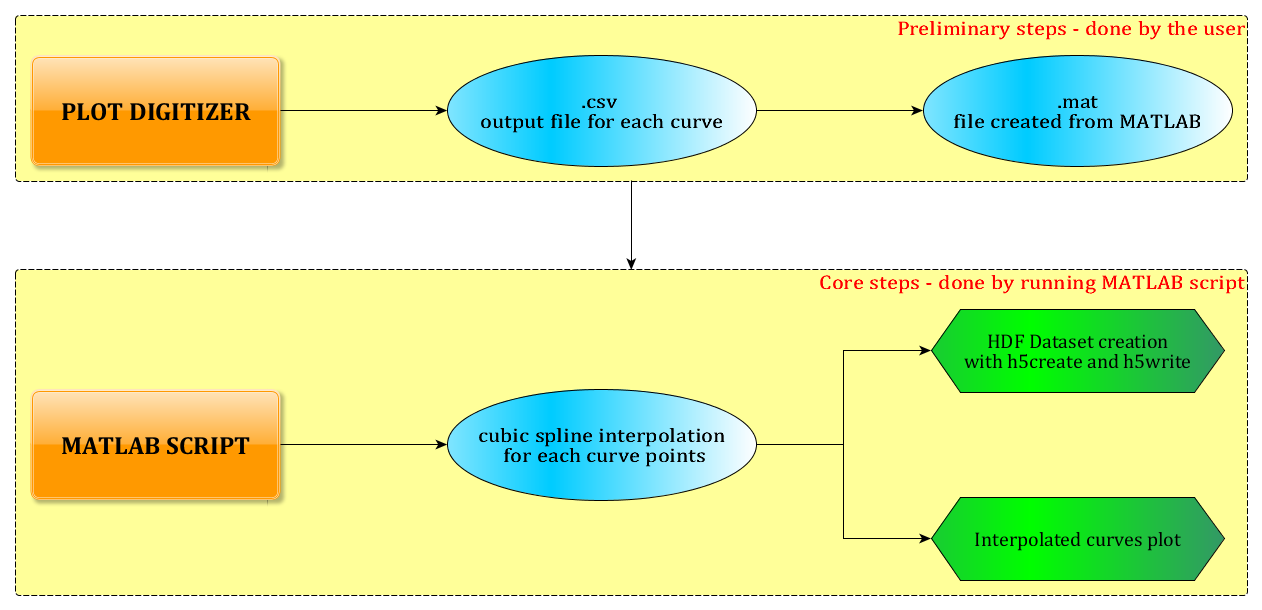
\includegraphics[keepaspectratio, width=0.88\textwidth]{HDF_Dataset_creation.png}
\caption{Flowchart of an HDF Database creation}
\end{figure}
%
\clearpage
\begin{figure}
\centering
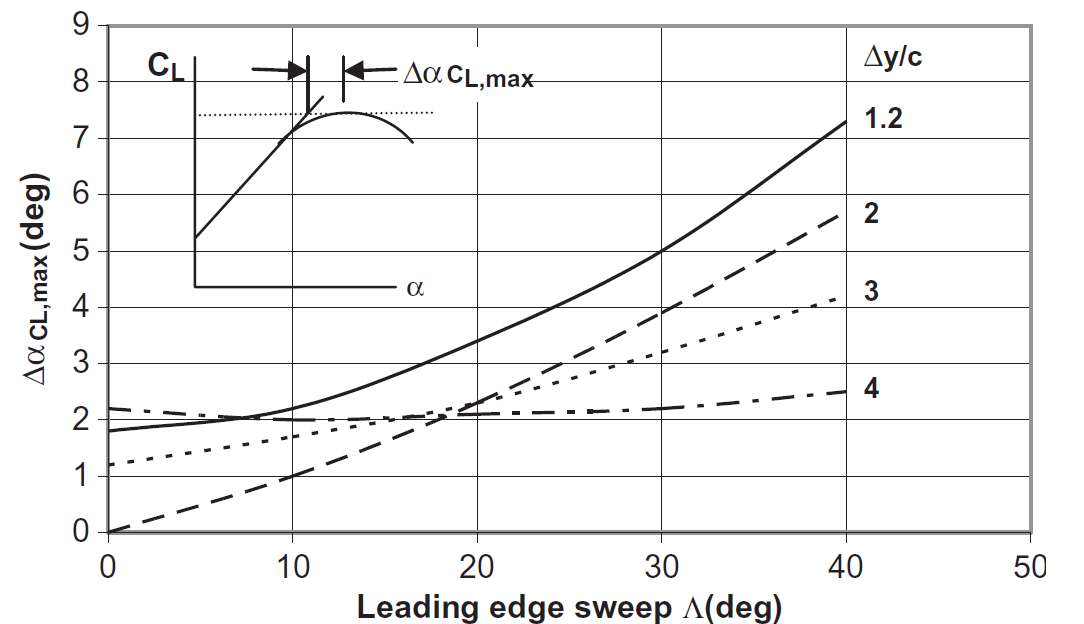
\includegraphics[keepaspectratio, width=0.55\textwidth]{deltaAlphaSforza.png}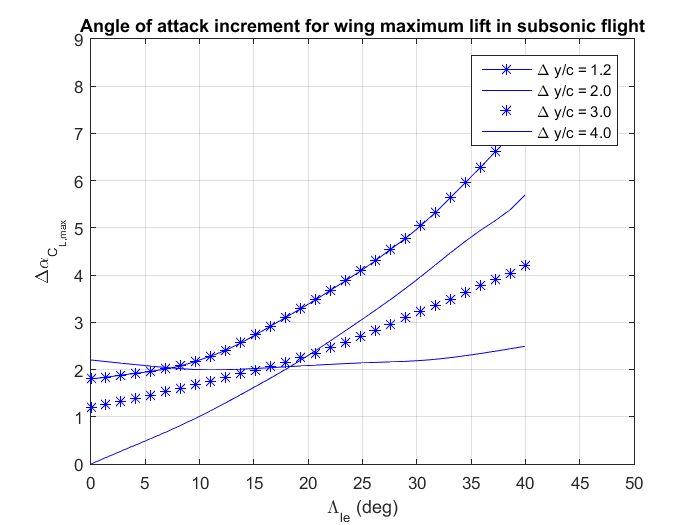
\includegraphics[keepaspectratio, width=0.55\textwidth]{DAlphaVsLambdaLEVsDy_MATLAB.png}
\caption{Comparison between the initial graph and the digitized one}
\label{fig:DeltaAlphaMaxClean}
\end{figure}
%
\section{Reading data from an HDF database in JPAD}\label{par:Appendix2}
After creating the database, this has to be read in order to obtain the required data; inside JPAD this operation can be done defining a specific class, which extends the abstract class \lstinline[language=Java]!DatabaseReader! that is designed for HDF dataset reading. 
%
This son class has a specific structure which main key points can be summarized in the following ones:
%
\begin{enumerate}
\item Creation of variables, in number equal to the function to be interpolated, using the type \lstinline[language=Java]!MyInterpolatingFunction! 
\item Creation of variables for all values that are wanted to be read from the interpolating functions
\item Creation of a constructor that accepts the folder path string and the file name string of the database. This constructor has to launch the interpolating method for all functions contained into the database by using  \lstinline[language=Java]!MyInterpolatingFunction! methods.
\item Creation of a getter method for each of the variables allocated at point 2 in order to obtain values from interpolated functions by giving in input the required parameters
\end{enumerate}
%
\noindent
In particular the class \lstinline[language=Java]!MyInterpolatingFunction! implements methods for a spline, bicubic and tricubic data interpolation as well as three methods for extracting a specific value from each of the previou interpolated curve.

\bigskip
\noindent
The following listing describes, with an example upon the aerodynamic database, how the reader class should be built up following the previous steps.
%
\lstset{language=Java}
\begin{lstlisting}[caption={DatabaseReader son class creation}, captionpos=t, tabsize=2]
public class AerodynamicDatabaseReader extends DatabaseReader {
// STEP 1:
	private MyInterpolatingFunction 
					c_m0_b_k2_minus_k1_vs_FFR,
					ar_v_eff_c2_vs_Z_h_over_b_v_x_ac_h_v_over_c_bar_v;
// STEP 2:
	double cM0_b_k2_minus_k1, ar_v_eff_c2;
// STEP 3:
	public AerodynamicDatabaseReader(String databaseFolderPath, String databaseFileName) {
		super(databaseFolderPath, databaseFileName);

		c_m0_b_k2_minus_k1_vs_FFR = 
						database.interpolate1DFromDatasetFunction(
										"(C_m0_b)_k2_minus_k1_vs_FFR"
						);
		ar_v_eff_c2_vs_Z_h_over_b_v_x_ac_h_v_over_c_bar_v =
						database.interpolate2DFromDatasetFunction(
										"(AR_v_eff)_c2_vs_Z_h_over_b_v_(x_ac_h--v_over_c_bar_v)"
										);
	}
// STEP 4:	
	public double get_C_m0_b_k2_minus_k1_vs_FFR(double length, double diameter) { 
		return c_m0_b_k2_minus_k1_vs_FFR.value(length/diameter);
	}
// STEP 4:
	public double get_AR_v_eff_c2_vs_Z_h_over_b_v_x_ac_h_v_over_c_bar_v(double zH, double bV, double xACHV, double cV) {
		return ar_v_eff_c2_vs_Z_h_over_b_v_x_ac_h_v_over_c_bar_v.value(zH/bV, xACHV/cV);
	}
}
\end{lstlisting}
%
\bigskip
\noindent
Once the class is created, is possible to create an object of it in any test class in order to have access to all its methods; in particular the user needs to invoke the getter related to the quantity he wants to read from the interpolating function. 